\chapter{Testy Funkcjonalne}
\section{Wstęp}
\section{Eliminacja zakłóceń sinusoidalnych}
\subsection{Integracja bloku filtra w projekcie}

W celu sprawdzenia integralności wykonanego bloku, zestawiono układ jak na Rysunku \ref{fig:itest}.
Test integracyjny ma wykazać czy występuje zgodność typów danych we/wyj oraz zgodność panelu konfiguracyjnego użytkownika.
Jeżeli nastąpi próba łączenia niekompatybilnych ze sobą bloków, wyświetli się błąd podobny do tego z Rysunku \ref{fig:error}.
Po podłączeniu bloków, środowisko nie zgłasza alarmów co oznacza, że filtr może przyjmować dane ze źródła USRP. 
Panel parametrów wyświetla się prawidłowo i wymaga od użytkownika podania kluczowych parametrów.
  
\begin{figure}[ht]
\centering
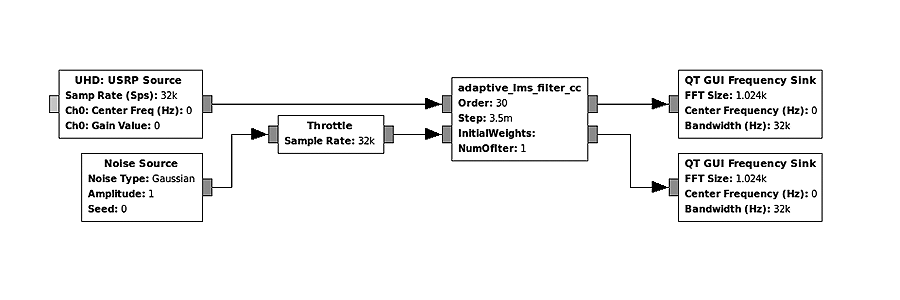
\includegraphics[scale=1.1]{ch5_integration.png}
\caption{Układ do testu integracyjnego}
\label{fig:itest}
\end{figure}


\begin{figure}[ht]
\centering
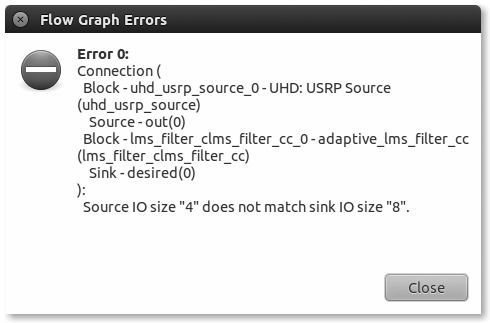
\includegraphics[scale=0.7]{ch5_error.png}
\caption{Błąd projektu informujący o niezgodności typów danych.}
\label{fig:error}
\end{figure}
\subsection{Weryfikacja poprawności działania}

\paragraph{Test 1.}
Wygenerowano szum pasmowy (od $2kHz$ do $3kHz$), który imituje sygnał danych.
Sygnał został zsumowany z falą zakłócającą o częstotliwości $2kHz$.
Suma została podana na wejście główne filtra, a do wejścia odniesienia podłączono źródło sygnału sinusoidalnego o tej samej częstotliwości, lecz innej fazie.
Częstotliwość sinusoid zwiększano stopniowo.

\paragraph{Obserwacja}
Na Wykresie \ref{fig:sine1} przedstawiono efekt filtracji sygnału.
Zakłócenie zostało pomyślnie odfiltrowane.

\begin{figure}[h]
\centering
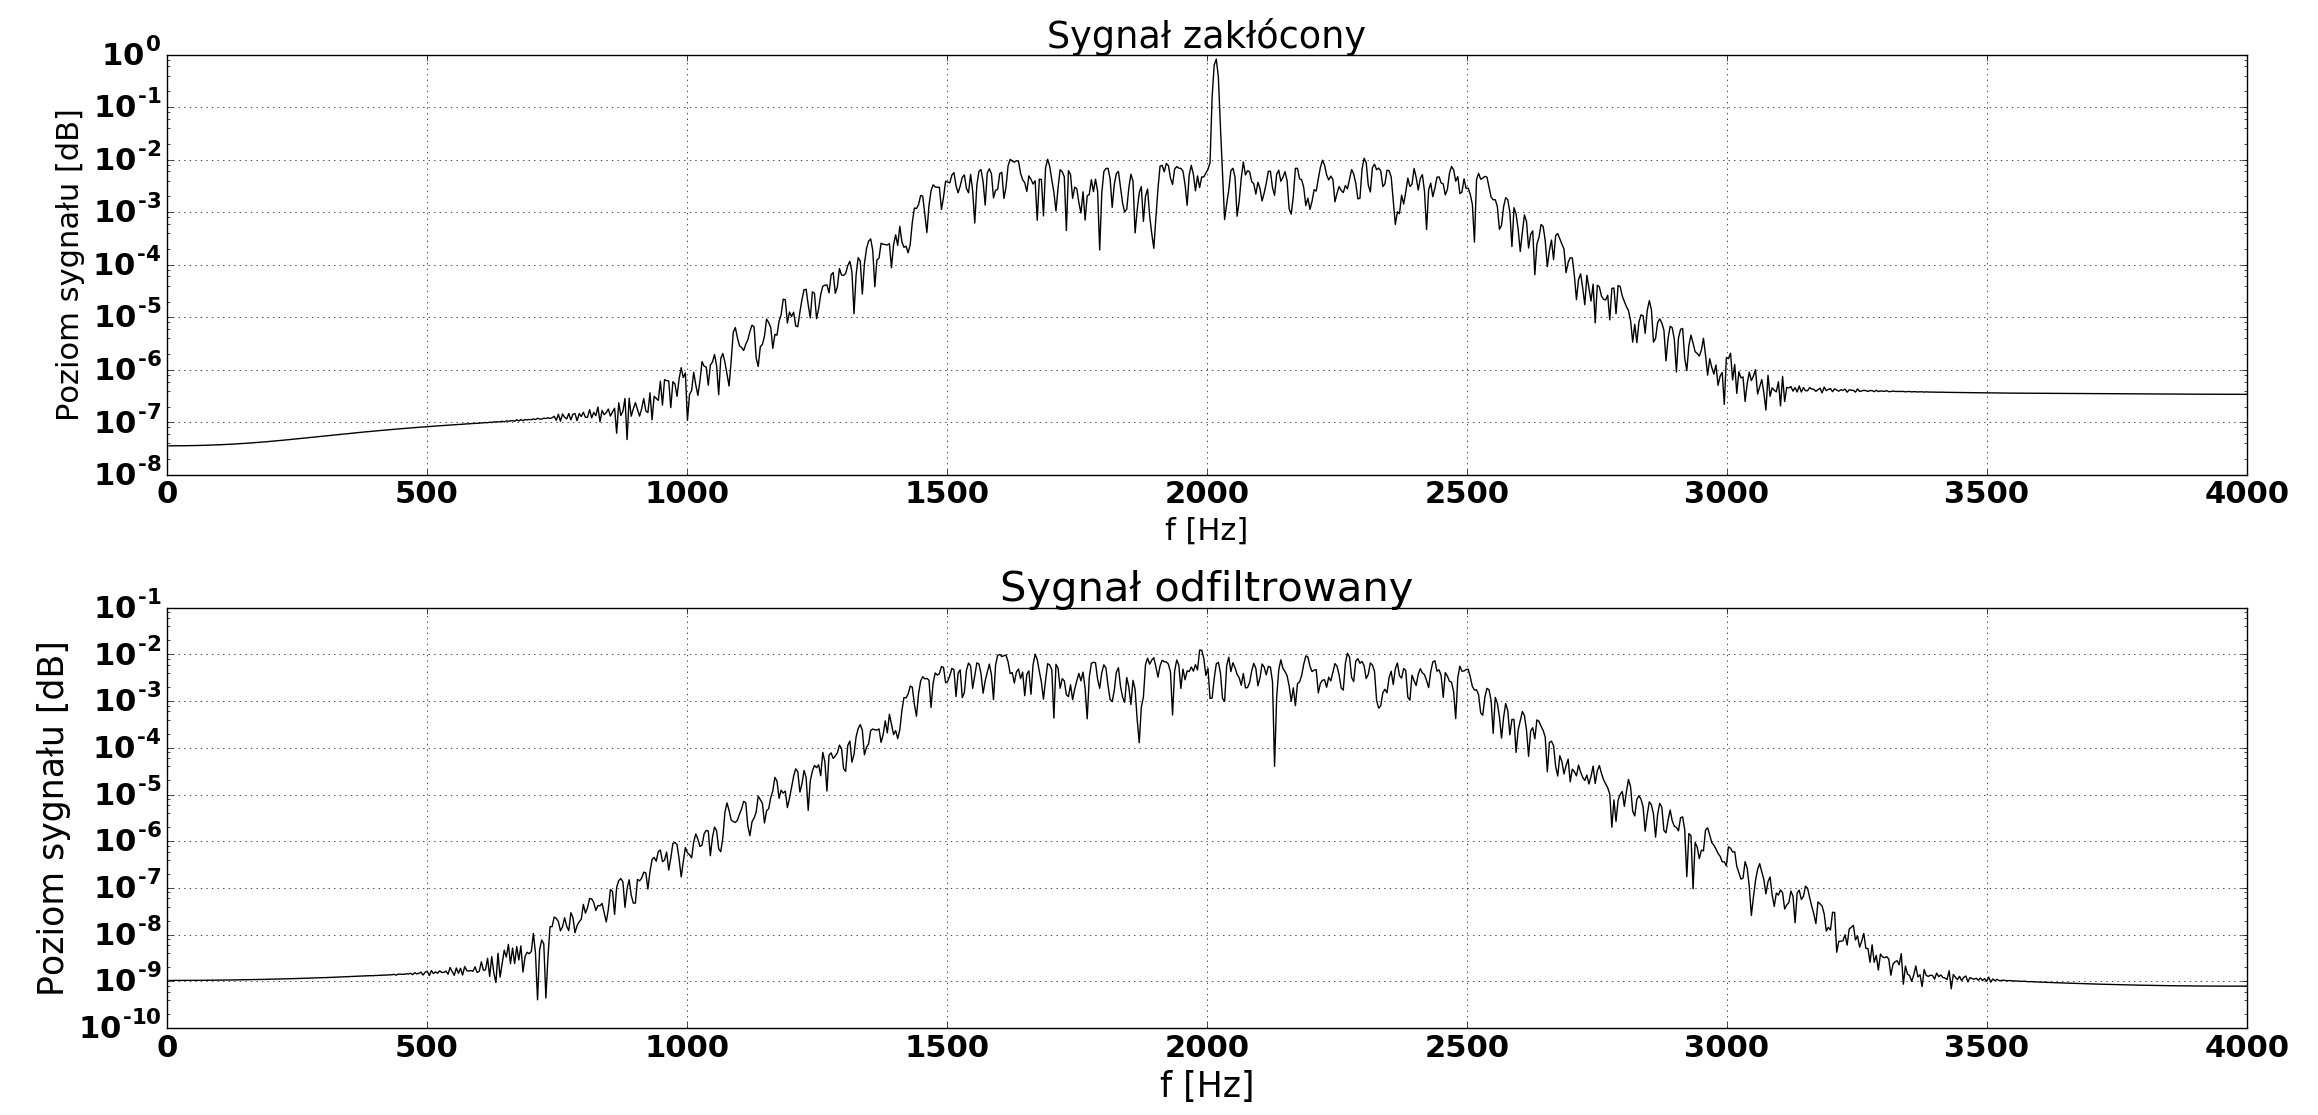
\includegraphics[scale=0.27]{sine1}
\caption{Filtracja zakłóceń o częstotliwości 2kHz}
\label{fig:sine1}
\end{figure}

\begin{figure}[h]
\centering
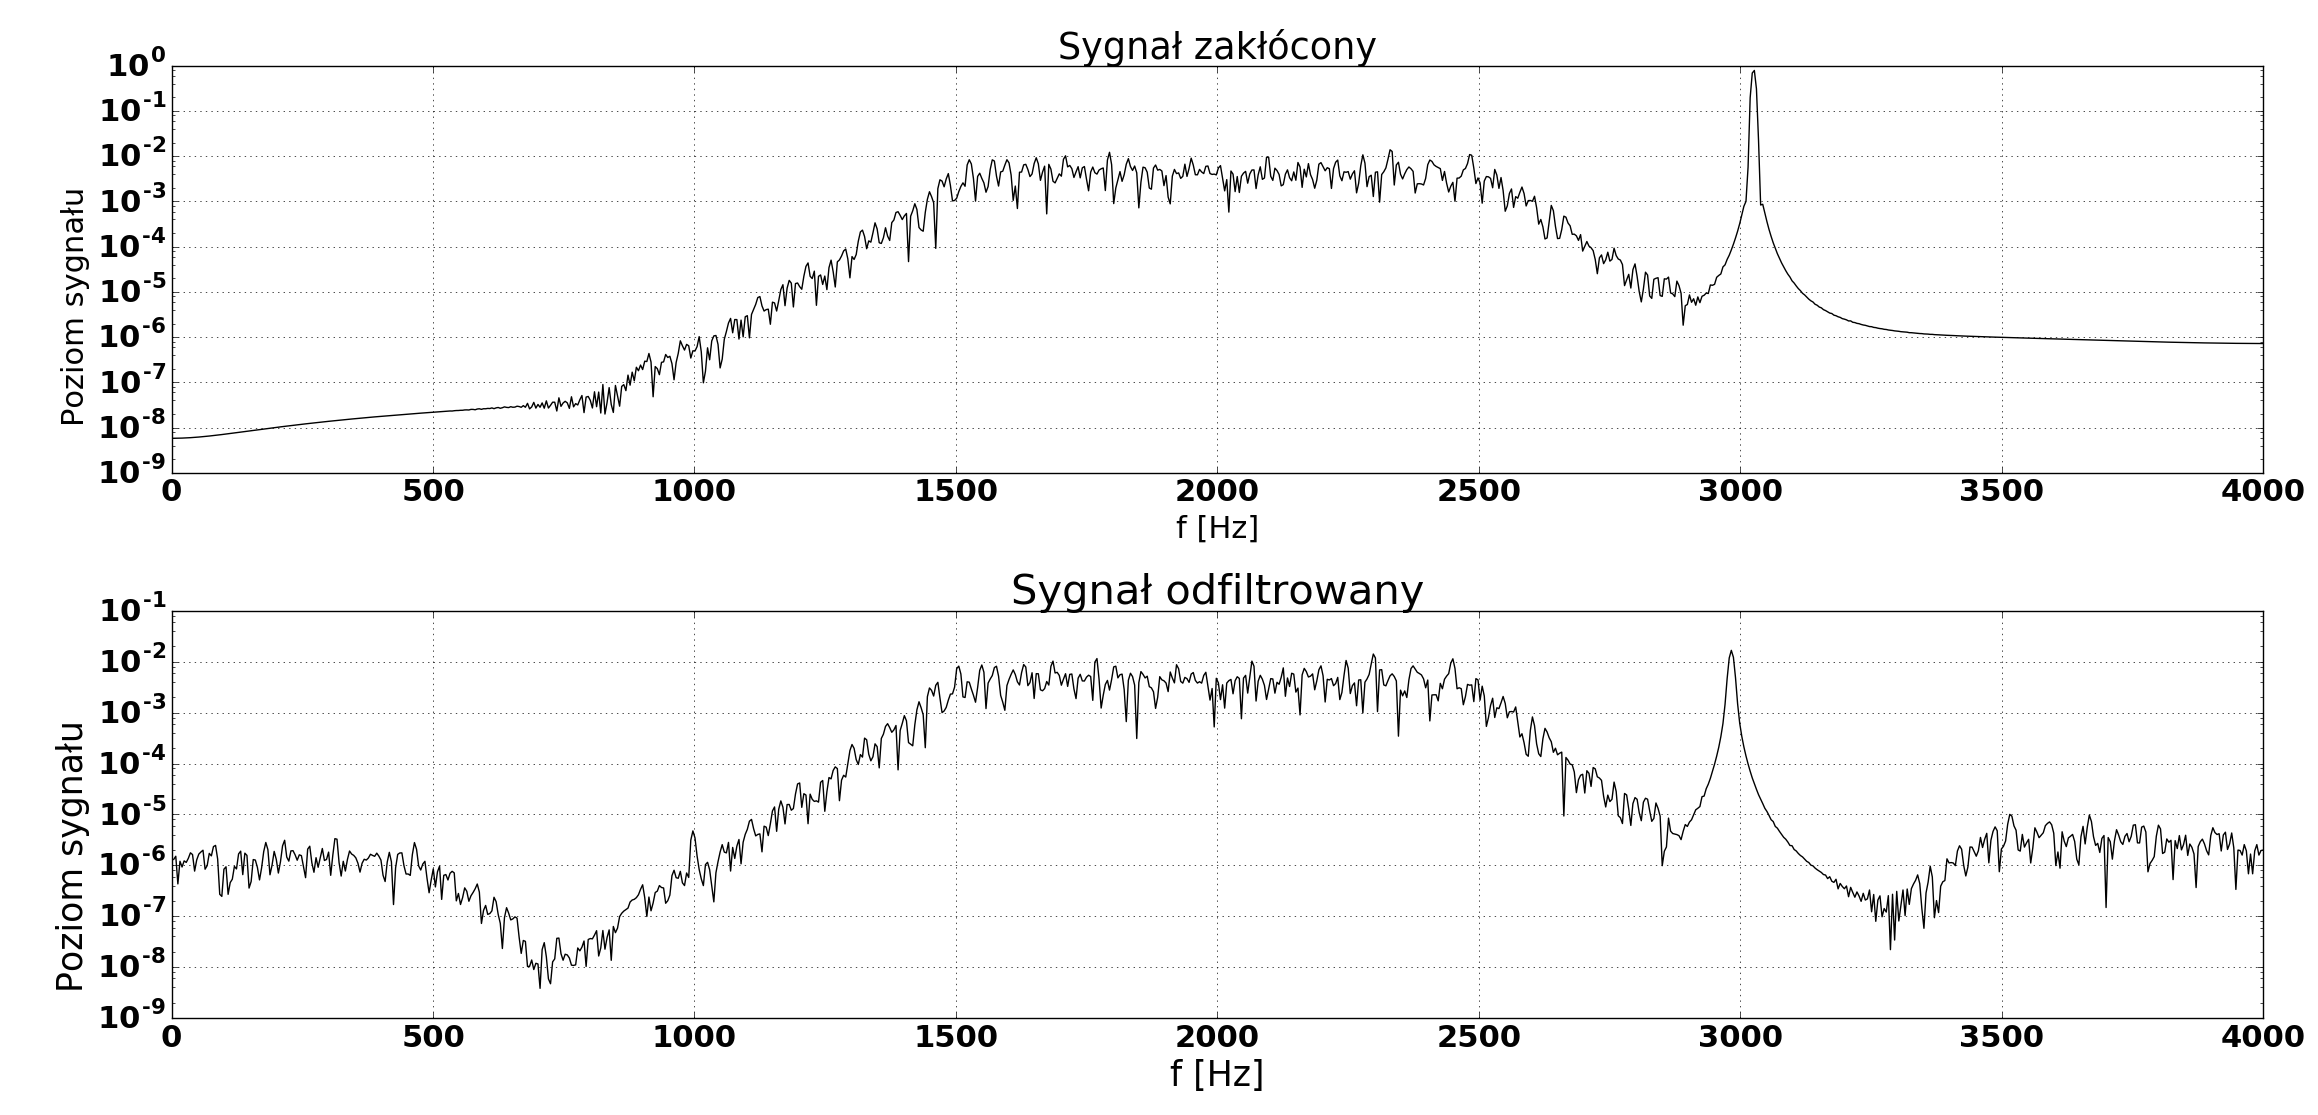
\includegraphics[scale=0.27]{sine2}
\caption{Filtracja zakłóceń o częstotliwości 3kHz}
\label{fig:sine2}
\end{figure}

Im większy jest parametr kroku $\mu$, tym szybsze są możliwości śledzenia przez filtr adaptacyjny (Rysunek \ref{fig:sine4}). Duży parametr kroku $\mu$ może sprowadzać niakceptowalnie duży błąd średniokwadratowy. \cite{Haykin:1998:ST} 
Przykładem tego są wyraźnie obserwowalne na rys. \ref{fig:sine3} zaniki w widmie, na częstotliwości odpowiadającej cz. sygnału zakłócającego.

\begin{figure}[h]
\centering
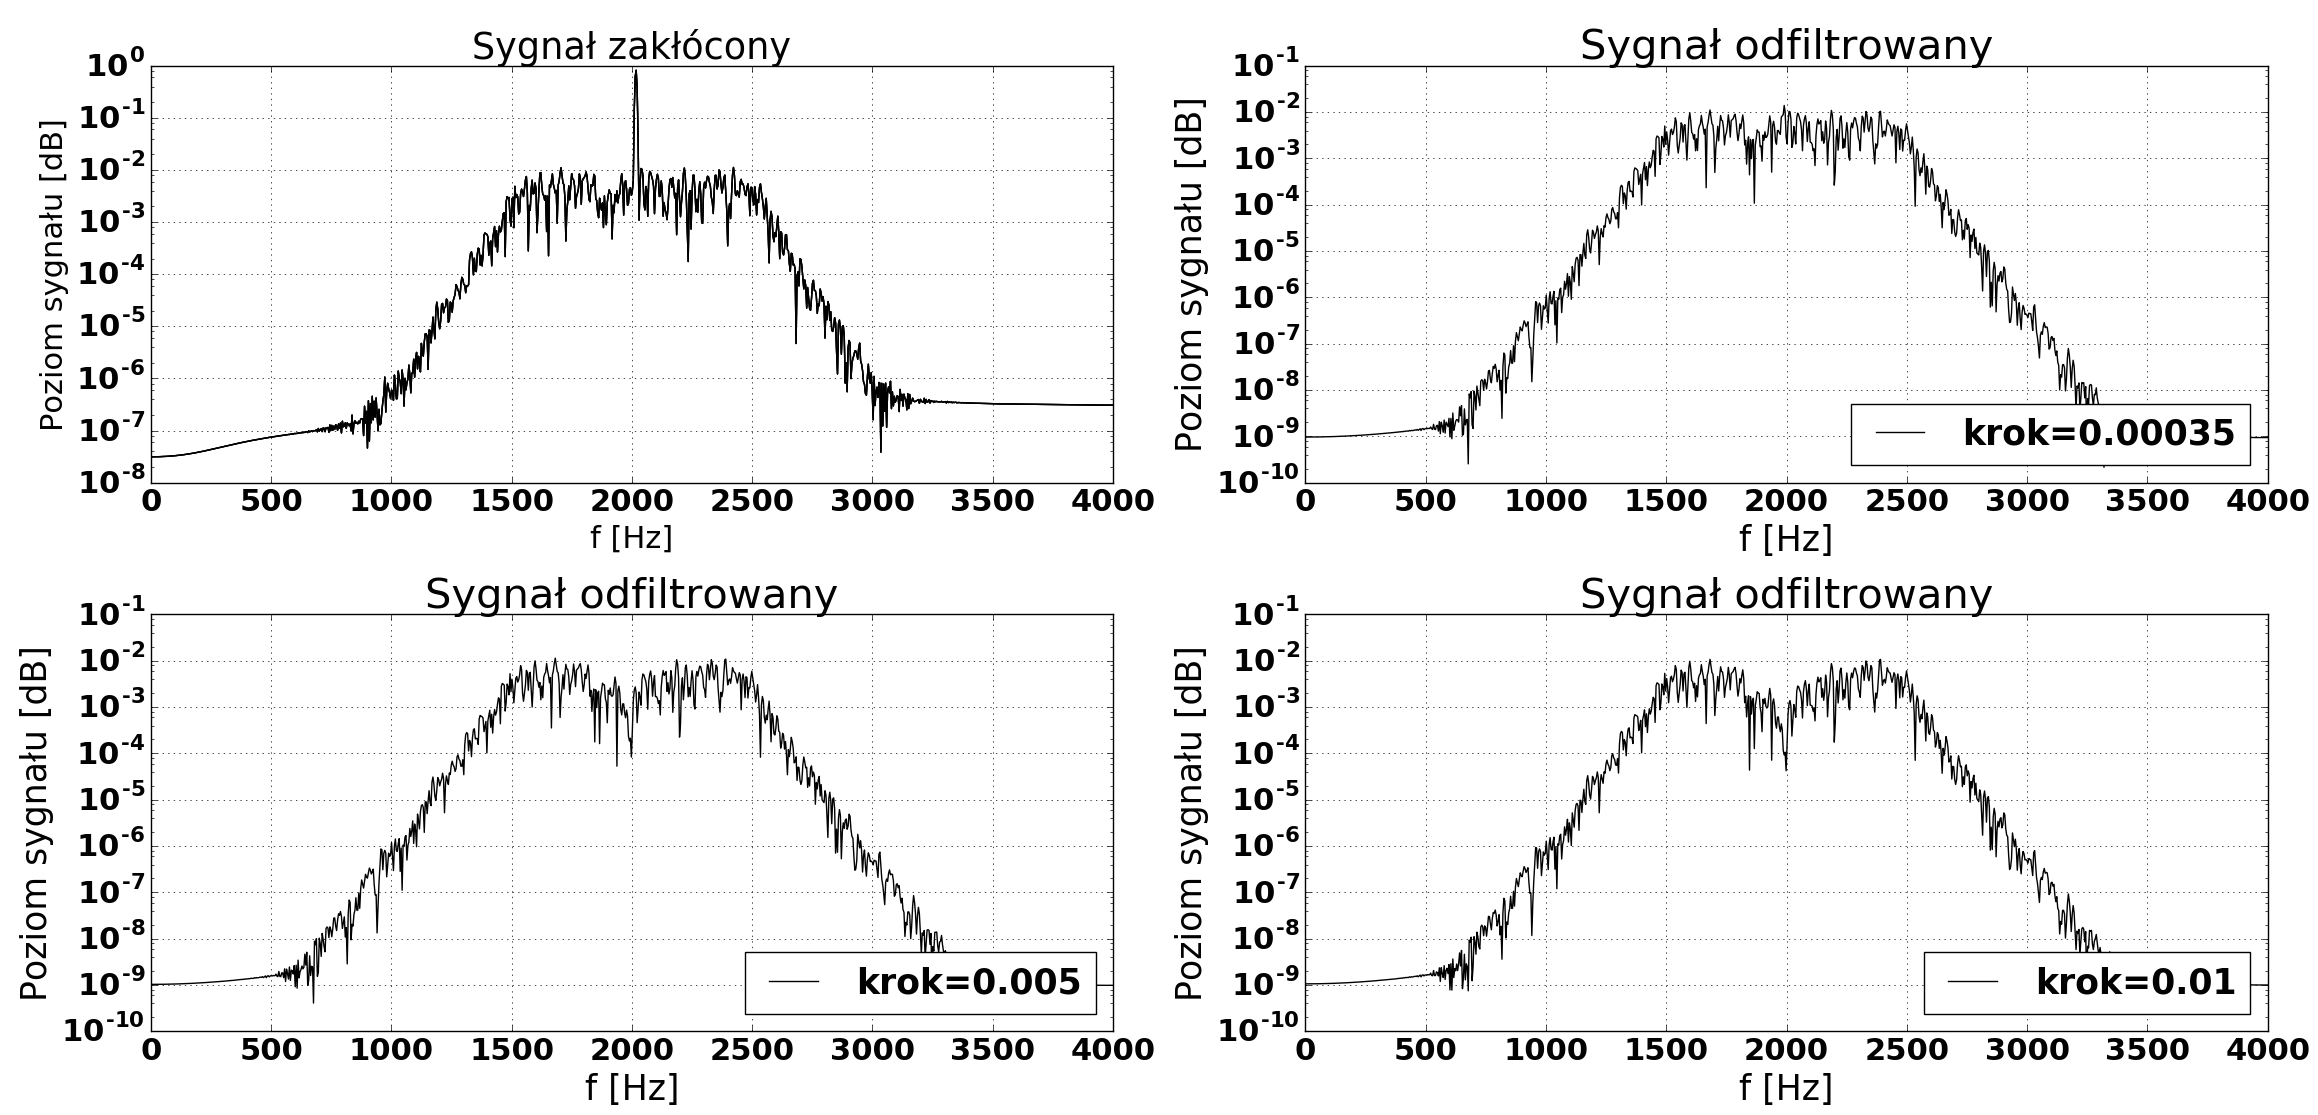
\includegraphics[scale=0.27]{sine3}
\caption{Wpływ parametru kroku na widmo sygnału.}
\label{fig:sine3}
\end{figure}

\begin{figure}[h]
\centering
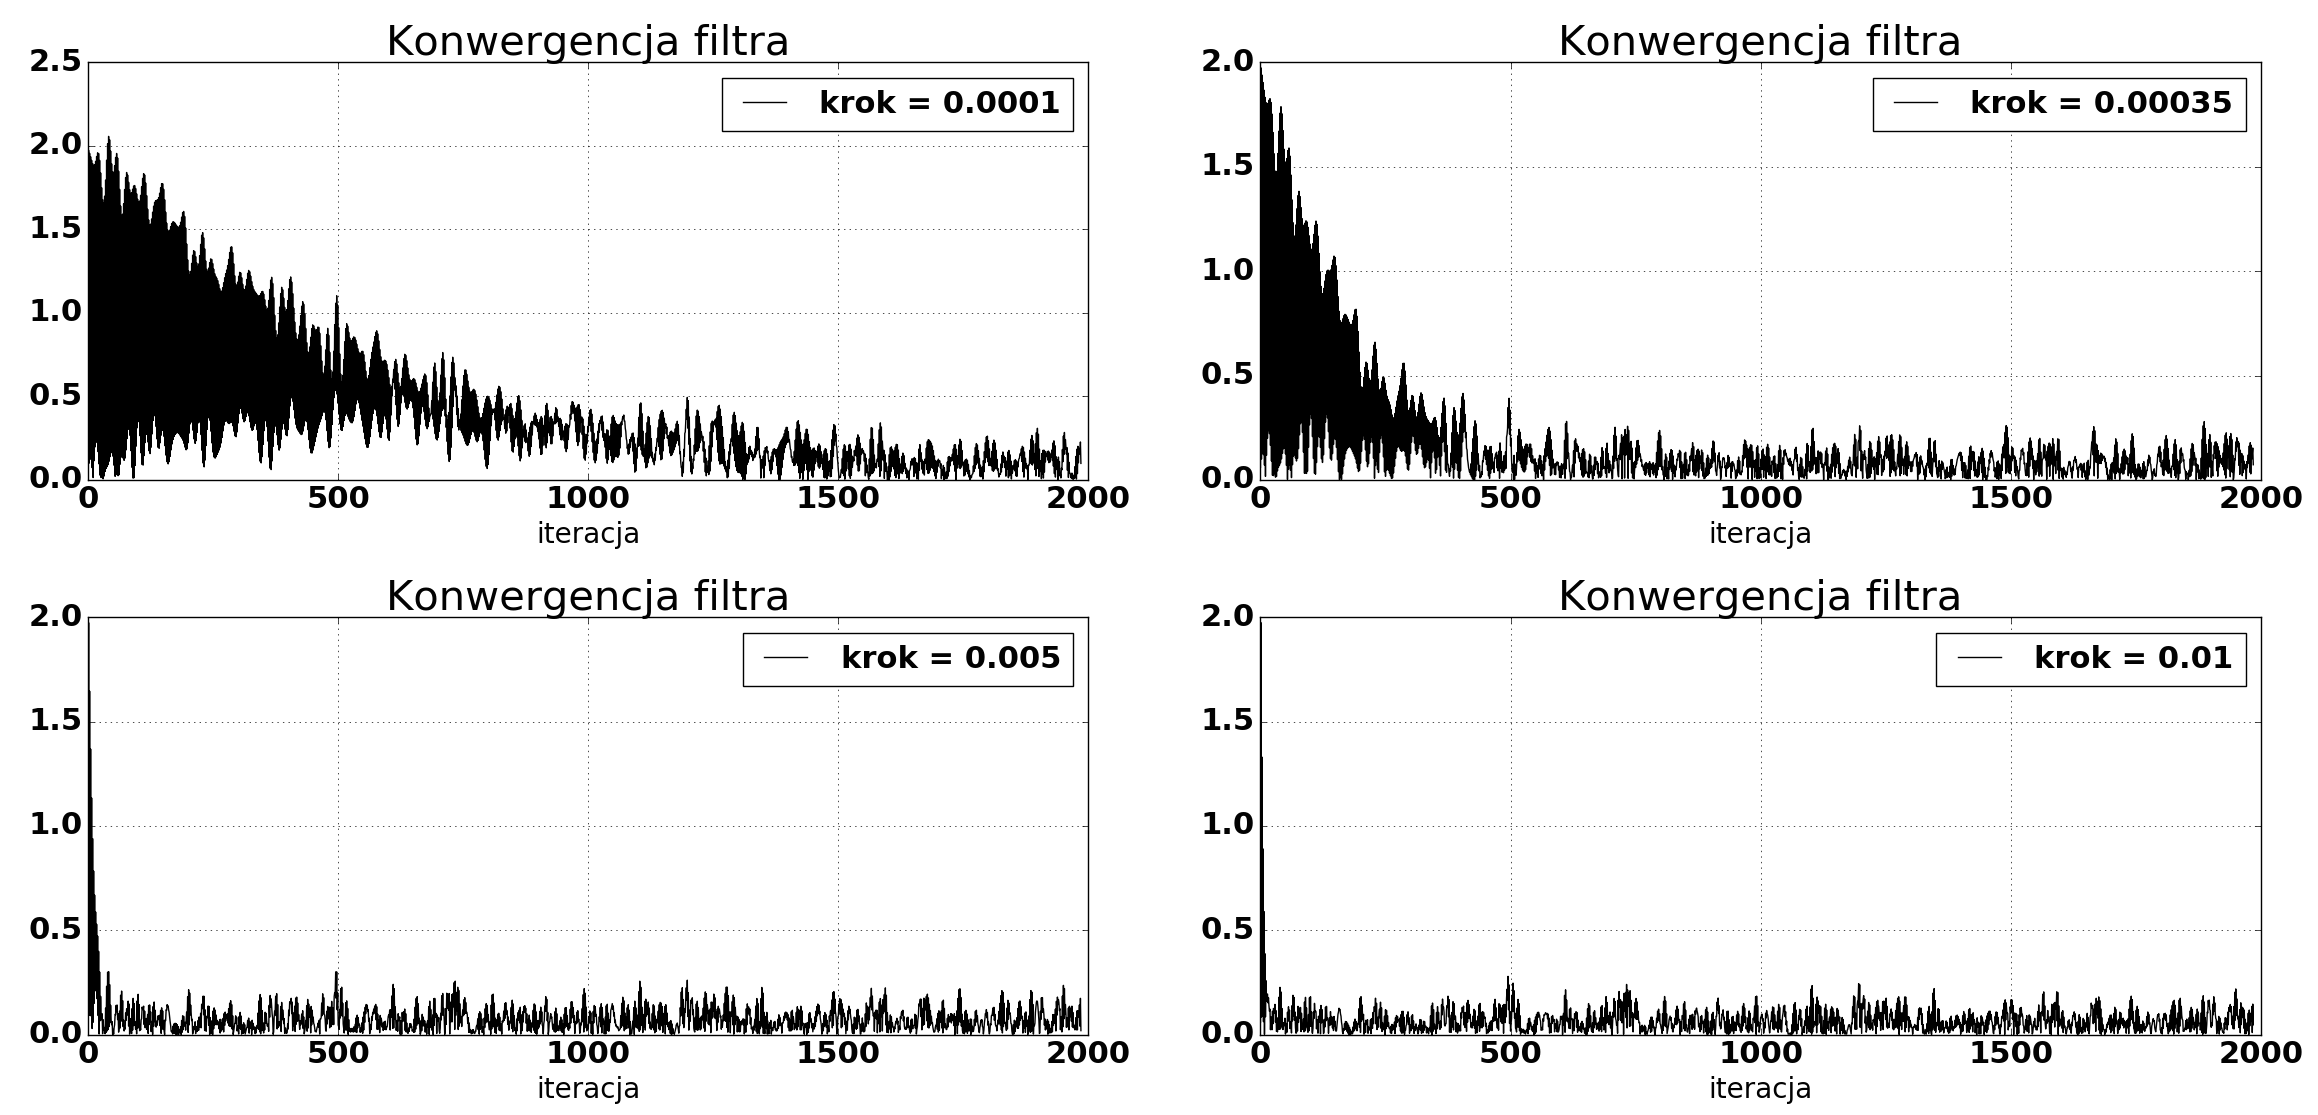
\includegraphics[scale=0.27]{konwergencja}
\caption{Wpływ parametru kroku na szybkość zbieżności algorytmu.}
\label{fig:sine4}
\end{figure}

\section{Korekcja adaptacyjna}

\begin{sidewaystable}[t]
\centering
\caption{My caption3}
\label{my-label3}
\begin{tabular}{l}
\hline
Transmisja bez korekcji \\
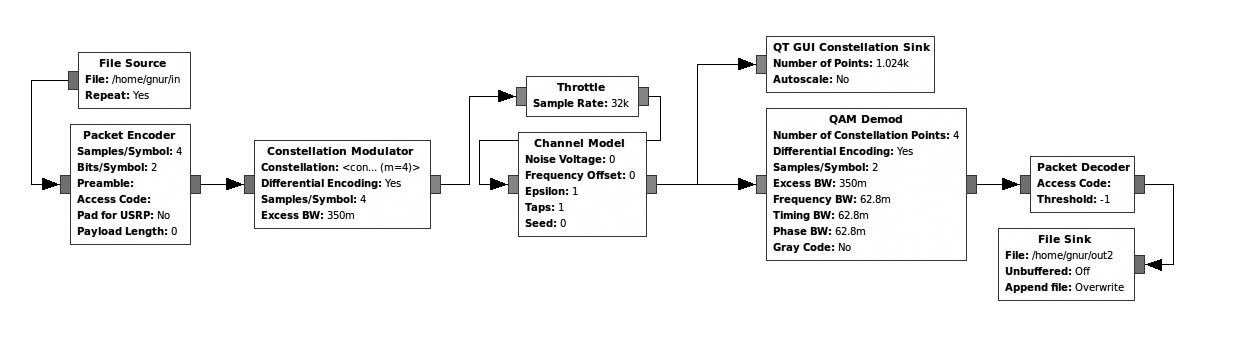
\includegraphics[scale=0.5]{noeq.png}\\ \hline
Transmisja z korekcją   \\
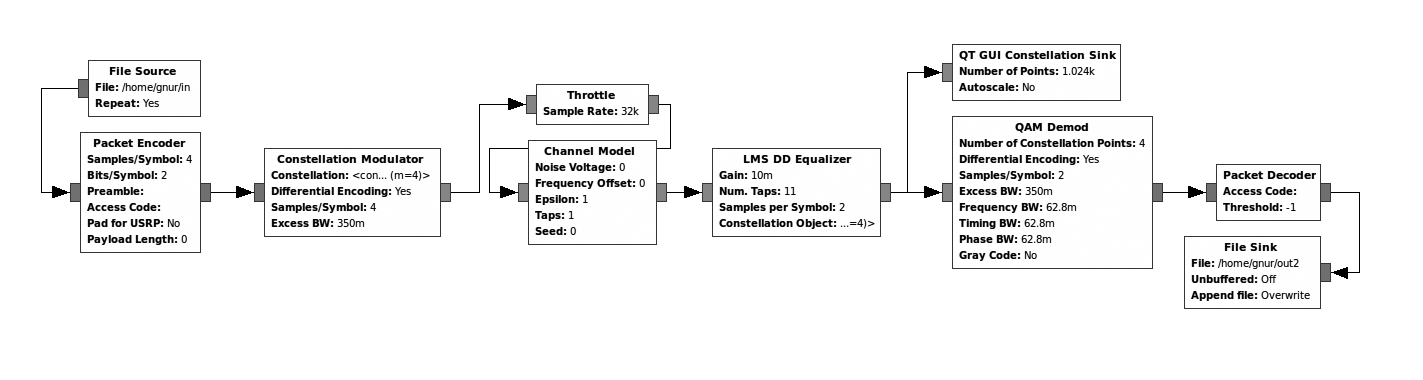
\includegraphics[scale=0.5]{eq.png}\\
\end{tabular}
\end{sidewaystable}

\begin{table}
\centering
\caption{My caption}
\label{my-label2}
\begin{tabular}{|l|l|l|}
\hline
0mV      & 150mV    & 200mV    \\
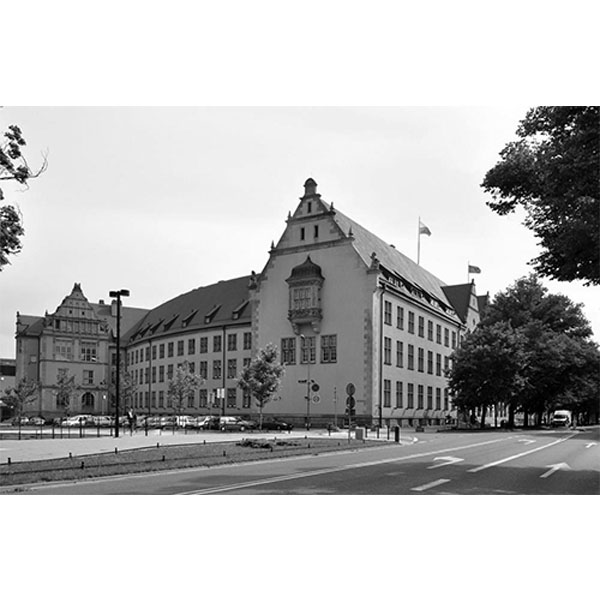
\includegraphics[scale=0.45]{a1origin} & 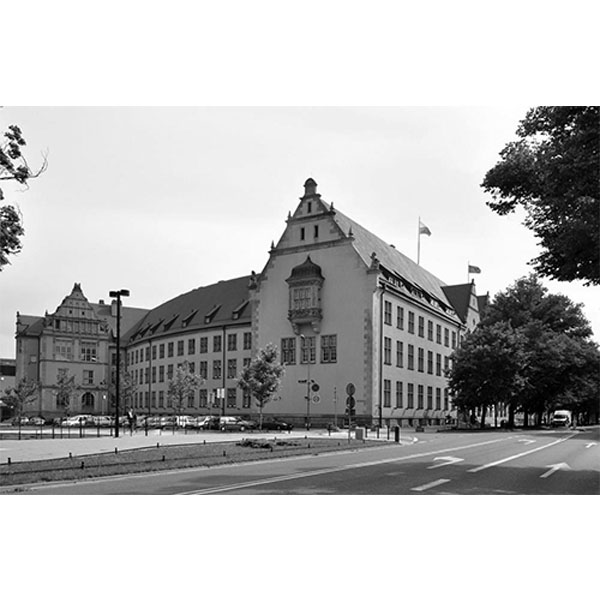
\includegraphics[scale=0.45]{a1origin} & 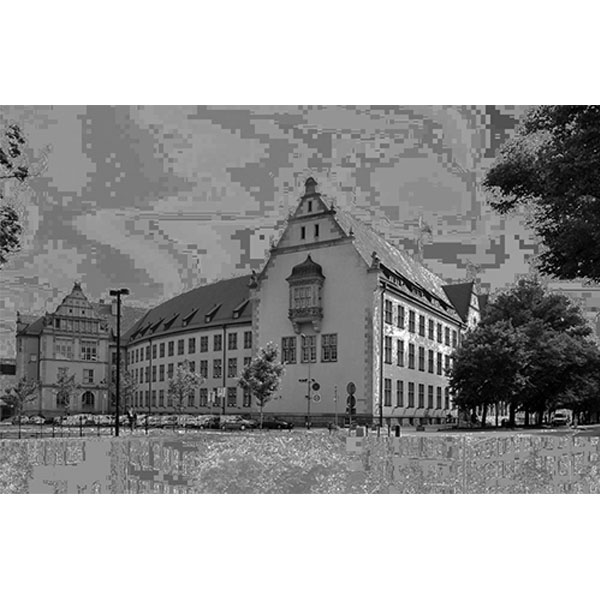
\includegraphics[scale=0.45]{noeq200mva1} \\
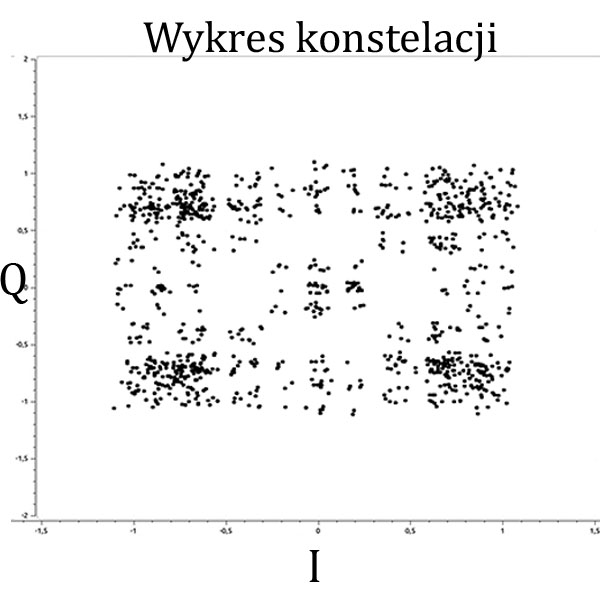
\includegraphics[scale=0.45]{noeq0mv}   & 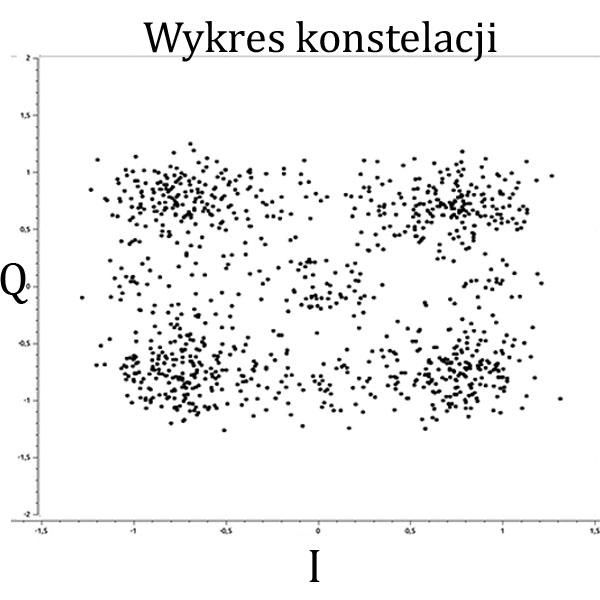
\includegraphics[scale=0.45]{noeq150mv}   & 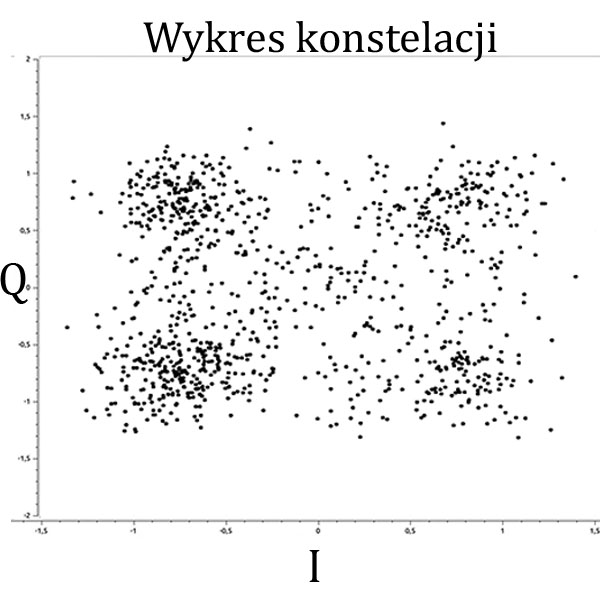
\includegraphics[scale=0.45]{noeq200mv}  \\ \hline
\end{tabular}
\end{table}


\begin{table}
\centering
\caption{My caption}
\label{my-label}
\begin{tabular}{|l|l|l|}
\hline
0mV      & 200mV    & 250mV    \\
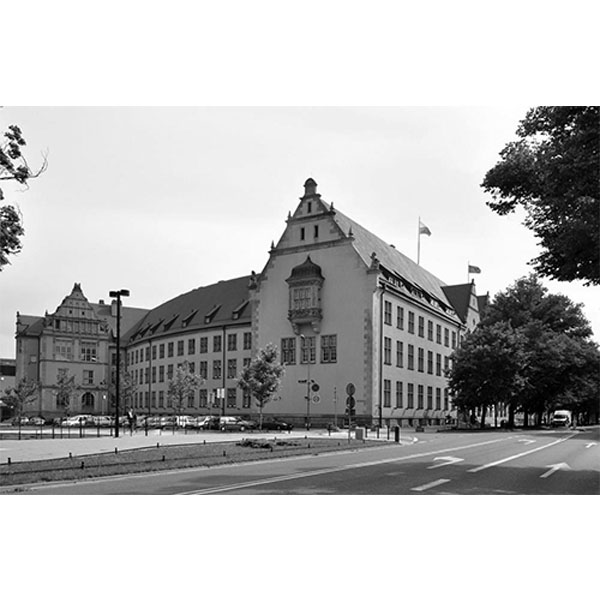
\includegraphics[scale=0.45]{a1origin} & 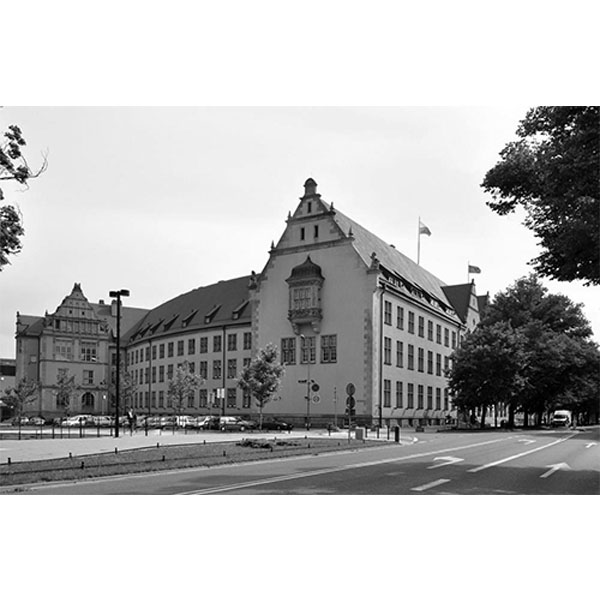
\includegraphics[scale=0.45]{a1origin} & 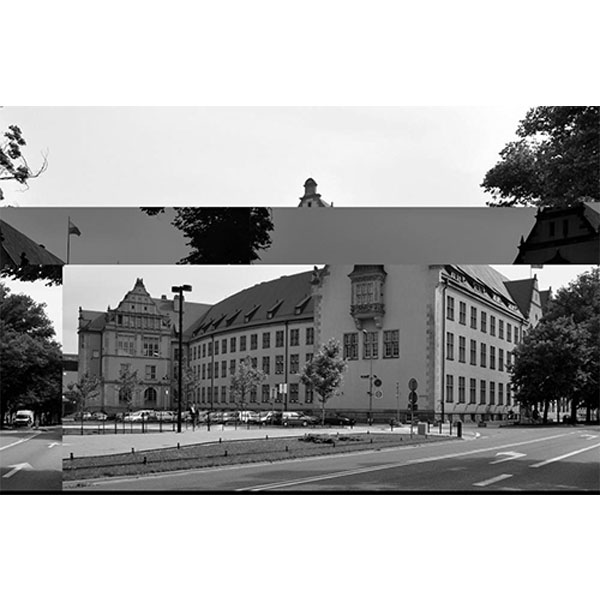
\includegraphics[scale=0.45]{eq250mva1} \\
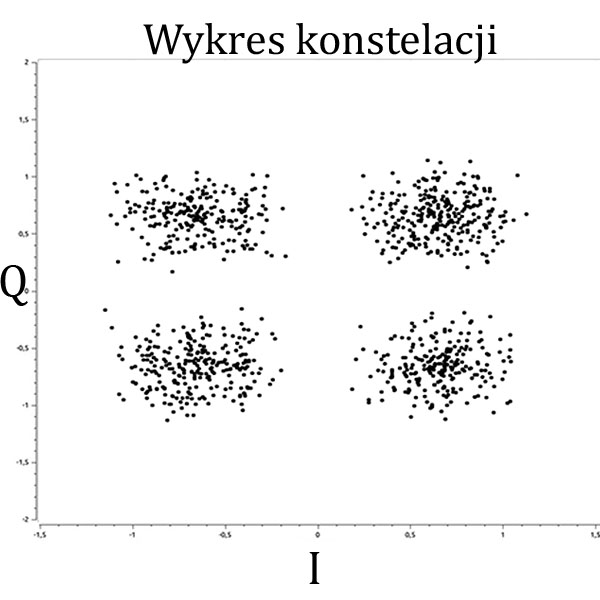
\includegraphics[scale=0.45]{eq0mv}   & 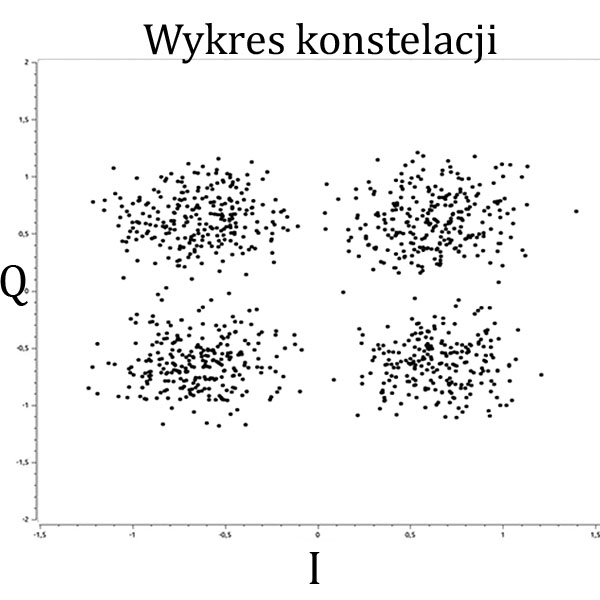
\includegraphics[scale=0.45]{eq200mv}   & 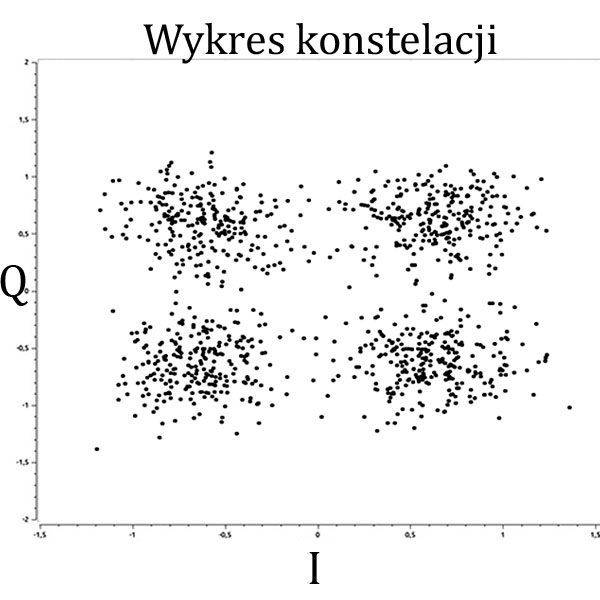
\includegraphics[scale=0.45]{eq250mv}  \\ \hline
\end{tabular}
\end{table}

\begin{table}[]
\centering
\caption{Korekcja kanału}
\label{channel_eq}
\begin{tabular}{|c|c|}
\hline
Kanał bez korekcji & Kanał z korekcją \\
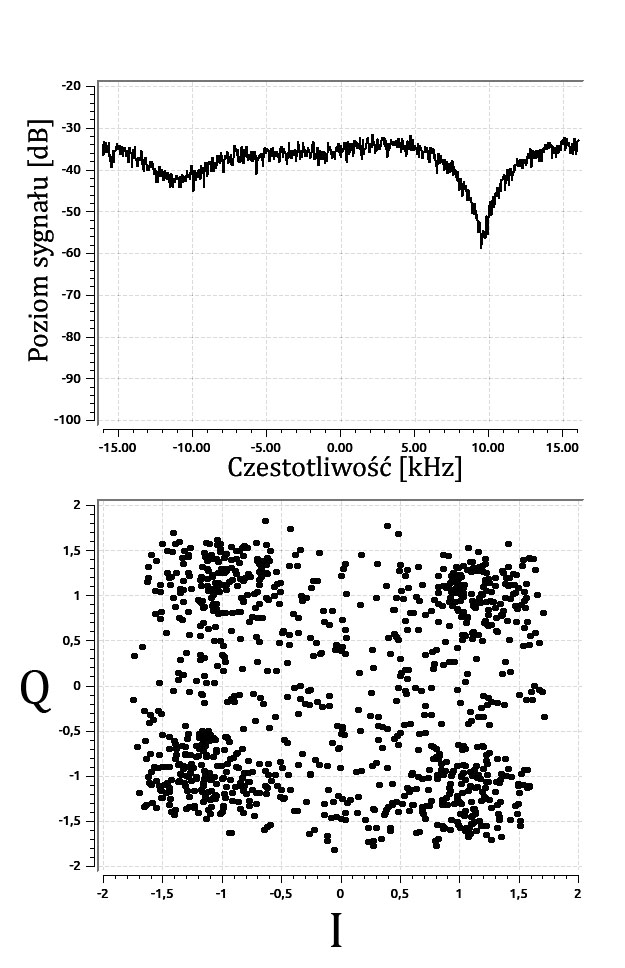
\includegraphics[scale=0.32]{channel_noeq}      & 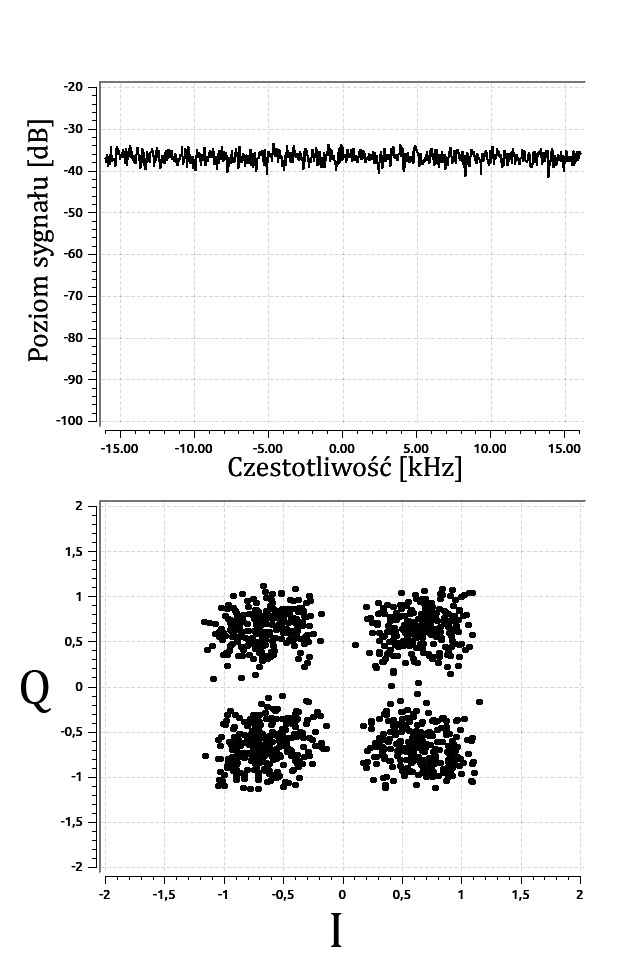
\includegraphics[scale=0.32]{channel_eq}      \\ \hline
\end{tabular}
\end{table}




